\documentclass[journal]{IEEEtran}
\usepackage{amsthm}
\newtheorem{definition}{Definition}

\usepackage{booktabs}
\usepackage[table]{xcolor}
\usepackage{pgfplots}
\pgfplotsset{compat=1.18}
%\usepackage{subcaption}
\usepackage{graphicx}
\usepackage{xcolor}
\usepackage{colortbl}
\usepackage{contour}
\contourlength{0.8pt} % thickness of the halo

\usepackage{amssymb}
%\usepackage{hyperref}
\usepackage[utf8]{inputenc}
%\usepackage[hidelinks]{hyperref}
\usepackage{url}
\usepackage{cite}
\usepackage{enumitem}
%\usepackage{subfig}
\usepackage{subfigure}
\usepackage{amsmath}
\usepackage{algorithm}
\usepackage{algpseudocode}
%\usepackage{caption}
\usepackage{pgf-pie}
\usepackage{pgfplots}
\usepgfplotslibrary{dateplot}
\usepgfplotslibrary{units}
\pgfplotsset{compat=1.18}
\usepackage{tabularx}
\usepackage{booktabs}
\usepackage{minted}
\usemintedstyle{borland}
\usepackage{comment}
\usepackage{pgf-pie}
\usepackage[obeyclassoptions,mode=buildnew]{standalone}

\usetikzlibrary{arrows.meta, positioning, calc}

% darken the colors a little bit
\definecolor{red}  {rgb}{0.9,0.0,0.0}
\definecolor{green}{rgb}{0.0,0.7,0.0}
\definecolor{blue} {rgb}{0.0,0.0,0.9}

\definecolor{OkabeBlue}{RGB}{0,114,178}
\definecolor{OkabeOrange}{RGB}{213,94,0}
\definecolor{OkabeGreen}{RGB}{0,158,115}
\definecolor{OkabeSky}{RGB}{86,180,233}
\definecolor{OkabeVermilion}{RGB}{230,159,0}

\definecolor{OIblue}{HTML}{0072B2}
\definecolor{OIorange}{HTML}{E69F00}
\definecolor{OIgrey}{HTML}{999999}

\newcommand{\arad}[1]{\textcolor{orange}{Arad: #1}}
\newcommand{\ori}[1]{\textcolor{blue}{Ori: #1}}
\newcommand{\discuss}[1]{\textcolor{blue}{#1}}
\newcommand{\red}[1]{\textcolor{red}{#1}}
\newcommand{\blue}[1]{\textcolor{green}{#1}}
\newcommand{\extended}[1]{}

\usepackage[most]{tcolorbox}

% \usepackage{authblk}

\title{Profitable Liquidity Provision: Mitigating DeFi Impermanent Loss}
\author{Arad Kotzer and Ori Rottenstreich}
%\institute{}

% \author{
% \IEEEauthorblockN{Arad Kotzer, Ori Rottenstreich}
% \IEEEauthorblockA{%\textit{Department of Computer Science } \\
% Technion - Israel Institute of Technology\\
% %Haifa, Israel \\
% emails: aradk@cs.technion.ac.il, or@technion.ac.il
% }
% }

\begin{document}

\maketitle

\begin{abstract}
Liquidity provision in automated market makers is often viewed as a passive income strategy. Though in practice, it can underperform buy-and-hold due to impermanent loss. This systematic shortfall arises when the relative prices of the pooled tokens diverge. In this paper, we propose a quantitative framework that evaluates this risk based on the historical divergence behavior of asset pairs rather than volatility summaries alone.

Analyzing 4.5 years of data from eight major Uniswap v3 pools, we construct an empirical risk profile that accounts for heavy-tailed outcomes. We report downside bounds and estimate the persistence of price divergence using mean-reversion half-life metrics. Our analysis reveals that correlation is more predictive of LP outcomes than headline volatility. Highly correlated pairs exhibit limited monthly drag even when individual assets are volatile, whereas stable--volatile pairs tend to incur more systematic erosion.
A recursive backtest shows that calibrated risk parameters transfer unevenly across pools, consistent with idiosyncratic divergence risk and departures from normality. 
These findings suggest that pool choice and holding horizon should be evaluated together, weighing expected fee income against both the distribution of IL risk and how long divergence typically persists.
\end{abstract}


%\keywords{Blockchain, DeFi, Impermanent Loss, Automated Market Makers}

\pagestyle{plain}
\thispagestyle{empty}

\section{Introduction}

The Decentralized Finance (DeFi) ecosystem comprises various financial services that run as blockchain applications~\cite{schar2021decentralized, zetzsche2020decentralized, jensen2021introduction, Bitcoin, wood2014ethereum}. DeFi enables participants to earn yield by providing services. The core strategies revolve around lending money for interest and providing liquidity to token exchanges for transaction fees. They also include generating actions on DeFi platforms to earn engagement rewards. Recent estimates of the DeFi token market cap range from approximately 90 billion USD~\cite{forbes2025defi} to 103 billion~\cite{coingecko2025defi}, as of December 2025.

However, the prevailing narrative that liquidity provision is a passive yield farming strategy is increasingly challenged by the reality of \textit{Impermanent Loss} (IL). IL represents the shortfall between the value of an LP’s pool position and the value of simply holding the same tokens (HODL). When the relative price of the two assets moves away from its initial level, the AMM automatically adjusts the pool’s reserve composition to satisfy its pricing rule. 
By doing so, it sells the outperforming asset and buys the underperforming one. 
As a result, the LP's total position value can end up below what they would have obtained by simply holding the assets outside the pool.


Empirical evidence suggests that for many LPs, the fee income generated is insufficient to compensate for this structural drag. 
Loesch et al.~\cite{loesch2021impermanent} study 17 popular Uniswap v2 pools and show that total fees earned (199M USD) failed to offset IL, resulting in an aggregate underperformance of 61M USD compared to the potential revenue of the HODL strategy (261M USD). 
These results imply a yield trap, as headline APYs look attractive, though after subtracting IL, fees often don’t cover the loss.

In this paper, \textit{we present a statistical framework for risk-aware pool selection and horizon management, weighing realized fee income against a full-range (CPMM) divergence-risk proxy computed from observed price ratios}. We analyze eight major Uniswap v3 pools over 4.5 years to characterize the stochastic behavior of price divergence. While prior studies focus on theoretical derivation, we introduce actionable, data-driven metrics to support decision-making under uncertainty.
Our analysis reveals that pools fall into distinct risk tiers driven by asset correlation rather than absolute volatility. We show that volatile--volatile pairs often exhibit lower IL risk than stable--volatile pairs due to high correlation. Based on these findings, we derive operational rules for pool selection, showing that maximizing fee velocity and matching horizons to statistical half-lives better predict net profit than the fee tier alone.
Our metric-guided pool selection yielded a total net gain of 77.38\%, outperforming simple pool averages and a HODL benchmark by over 30\%.


% The paper is structured as follows. Section~\ref{sec:background} provides the necessary background on AMMs and IL. Section~\ref{sec:metrics} introduces our statistical methodology, defining the mean-variance, non-parametric percentile, and mean-reversion metrics used to evaluate LPs risks. Section~\ref{sec:empirical_analysis} presents the empirical analysis of eight real-world Uniswap v3 pools, applying these metrics to historical data to uncover risk tiers and temporal dynamics. Section~\ref{sec:discussion} discusses the practical implications of these findings, proposing operational rules for pool selection and demonstrating their economic impact through a comparative case study. Finally, Section~\ref{sec:conclusion} concludes the paper and outlines directions for future research.



\section{Background and Related Work}
\label{sec:background}

\subsection{AMM (Automated Market Maker)}
Automated Market Makers (AMMs)~\cite{hertzog2017bancor} are decentralized exchange protocols that enable coin exchange using liquidity pools. 
The most common type of AMM is \emph{constant function market makers} (CFMMs). In CFMMs, token reserves $x_0, x_1$ are governed by a trading function $f(x_0,x_1)$ that imposes an invariant on these reserves.
The most prominent example is the constant-product rule $x_0 \cdot x_1 = K$ used by Uniswap v2. Generalizations include weighted geometric means (Balancer) and stableswap hybrids that blend constant product and sum (Curve)~\cite{bartoletti2022theory}.

AMMs operate as continuous, on-chain price discovery mechanisms driven by arbitrage flow. Whenever the pool price deviates from external markets, arbitrage restores alignment~\cite{angeris2020improved}. 
Hence, arbitrage creates a stabilizing mechanism and a source of value extraction~\cite{pusceddu2024lean}.
This arbitrage-based alignment sustains on-chain liquidity and also determines value transfers. %Traders may pay \emph{slippage} (execution worse than the pre-trade marginal price), and LPs may incur IL when the post-trade reserve mix underperforms HODL. Moreover, adversarial ordering (front-running, sandwiching~\cite{heimbach2022eliminating, zhou2021high}) can extract value under \emph{maximal extractable value} (MEV) \cite{mazorra2022price, daian2020flash, qin2021mev}.

\subsection{Liquidity Provision}
\label{sec:liquidity-provision}

Liquidity provision refers to users depositing tokens into an AMM pool, enabling traders to swap assets directly against pooled reserves. In return, \textit{liquidity providers} (LPs) receive a proportional share of the pool’s swap fees~\cite{gogol2024sok, chiu2023fragility, saengchote2023decentralized}.
For example, in a pool of Uniswap v2 ETH / USDC, LPs deposit equal values of ETH and USDC. Traders then exchange one asset for the other via the constant product invariant of the pool. This mechanism underpins decentralized exchanges by providing continuous on-chain liquidity without order books.
%Fig.~\ref{fig:pool_illustration} illustrates the liquidity provision flow. First, an LP deposits amounts $(x_0,x_1)$ of assets $(c_0,c_1)$ into the pool. When a trader swaps, the pool balances change along the pricing curve, updating the implied price. Finally, upon withdrawal, the LP receives her new proportional mix of tokens plus the fees accrued to the position.

% \begin{figure}[h]
% \centering
% \resizebox{\linewidth}{!}{%
% \begin{tikzpicture}[
%   >={Stealth[length=3mm]},
%   node distance=2.2cm,
%   pool/.style={rectangle, rounded corners, draw, thick, minimum width=4cm, minimum height=1.6cm, align=center},
%   role/.style={rectangle, draw, rounded corners, minimum width=2.4cm, align=center},
%   lab/.style={font=\footnotesize}
% ]
% % Nodes
% \node[role] (lp) {Liquidity Provider (LP)};
% \node[pool, right=3.6cm of lp] (amm) {AMM Pool\\rebalancing by invariant};
% \node[role, right=3.6cm of amm] (trader) {Trader};

% % LP deposit & LP tokens
% \draw[->, thick] (lp.east) -- node[lab, above] {deposit $x_0, x_1$} (amm.west);
% % \draw[<-, thick] ($(amm.west)+(0, -0.35)$) -- node[lab, below] {mint LP tokens} ($(lp.east)+(0, -0.35)$);

% % Trader swap & fees
% \draw[->, thick] (trader.west) -- node[lab, above] {swap $\Delta x_0 \leftrightarrow \Delta x_1$} (amm.east);
% % \draw[->, thick, shorten >=2pt] ($(amm.east)+(0,-0.35)$) -- ++(0.9, -0.7)
% %   node[lab, right, align=left] {fees accrue\\to pool};

% % Withdraw
% \draw[<-, thick, bend right=20] (lp.south) to node[lab, below, align=center] {withdraw new mix\\($x'_0, x'_1$) + fees} (amm.south);

% % Annotations inside pool
% \node[lab] at ($(amm.north)+(0,0.25)$) {price $P = x_1/x_0$};
% \end{tikzpicture}%
% }
% \caption{Liquidity provision illustration of a constant-product AMM}
% \label{fig:pool_illustration}
% \end{figure}


\begin{figure}[t!]
\centering
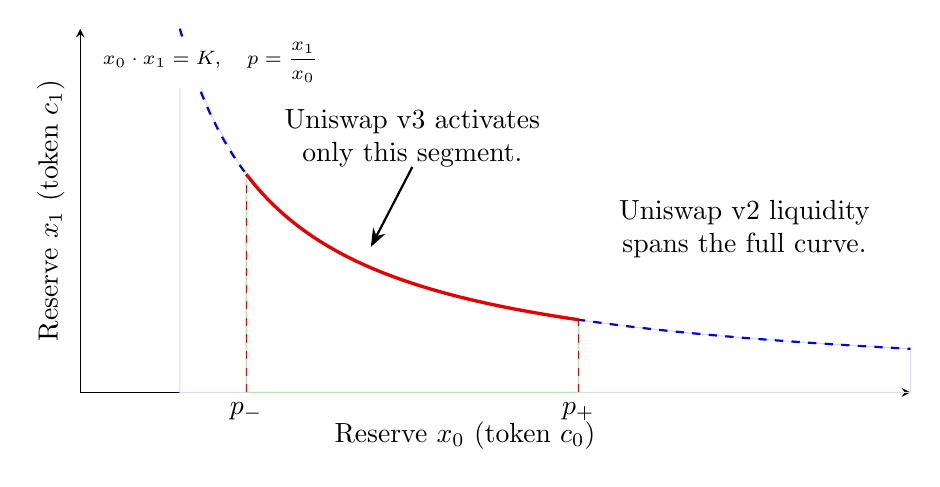
\begin{tikzpicture}[
  fill_v2/.style={blue!15, fill opacity=0.8},
  fill_v3/.style={green!30, fill opacity=0.8},
  plot_curve/.style={blue, thick},
  highlight_curve/.style={red, very thick},
]
\begin{axis}[
  xlabel={Reserve $x_0$ (token $c_0$)},
  ylabel={Reserve $x_1$ (token $c_1$)},
  axis lines=left,
  xmin=0, xmax=10,
  ymin=0, ymax=10,
  width=\linewidth, height=6.2cm,
  xtick=\empty, ytick=\empty,
  enlargelimits=false,
  clip=false,
  xlabel style={anchor=north, yshift=-5pt, xshift=-11pt},
  ylabel style={anchor=south},
]
% price band:
\def\pmin{2}
\def\pmax{6}

% v2 (full range)
\addplot [fill_v2, domain=1.2:10] {12/x} \closedcycle;

% v3 (concentrated range)
\addplot [fill_v3, domain=\pmin:\pmax] {12/x} \closedcycle;

% full bonding curve
\addplot [plot_curve, dashed, domain=1.2:10, samples=100] {12/x};

% active v3 segment
\addplot [highlight_curve, domain=\pmin:\pmax, samples=100] {12/x};

% price band markers
\draw[red, dashed] (axis cs:\pmin, 0) node[below=0.01pt, black] {\(p_{-}\)} -- (axis cs:\pmin, {12/\pmin});
\draw[red, dashed] (axis cs:\pmax, 0) node[below=0.01pt, black] {\(p_{+}\)} -- (axis cs:\pmax, {12/\pmax});

% labels (avoid “price” wording)
\node[text width=3.2cm, align=center] at (axis cs:8,4.5)
  {Uniswap v2 liquidity spans the full curve.};
\node[text width=3.5cm, align=center] at (axis cs:4,7)
  {Uniswap v3 activates only this segment.};
\draw[-Stealth, thick] (axis cs:4,6.2) -- (axis cs:3.5,4);

% small note: price definition
\node[anchor=north west, font=\scriptsize, fill=white, rounded corners=1pt, inner sep=2pt]
  at (rel axis cs:0.02,0.98) {$x_0 \cdot x_1=K,\quad p=\dfrac{x_1}{x_0}$};
\end{axis}
\end{tikzpicture}
\caption{Liquidity distribution in Uniswap v2 (full range) vs.\ Uniswap v3 (concentrated in \([p_{-},p_{+}]\)). The curve shows a constant-product contour \(x_0 \cdot x_1=K\), and the highlighted segment marks the price band where v3 liquidity is active.}
\label{fig:uniswap_fee_policy}
\end{figure}

\subsubsection{Fee microstructure and concentrated liquidity}
AMM protocols differ in how fees interact with liquidity.
In Uniswap v2, swap fees are \emph{reinvested into the pool reserves} on each trade, so the product $x_0 \cdot x_1{=}K$ grows.
In Uniswap v3, fees are added to the \emph{separate fee counters} of each position and do not change the active liquidity or the reserves until the LP explicitly claims or reinvests them.
Moreover, v3 allows LPs to choose a price band $[p_{-},p_{+}]$ and provide liquidity only inside it, as illustrated in Fig.~\ref{fig:uniswap_fee_policy}.
Let $p_{\text{pool}}$ denote the instantaneous pool price implied by reserves, defined as
$p_{\text{pool}} = x_1/x_0$. 
When $p_{\text{pool}}\in[p_{-},p_{+}]$, the position behaves locally like a Constant Product Market Maker (CPMM) with ``virtual'' reserves determined by $[p_{-},p_{+}]$ and its liquidity $L$, and it earns fees. 
If price exits this band, the position becomes out of range and is held entirely in a single asset, $c_0$ when $p_{\text{pool}}<p_{-}$ and $c_1$ when $p_{\text{pool}}>p_{+}$. 
In this out-of-range state, the position provides no active liquidity and therefore accrues no fees until the price re-enters the range or the LP rebalances.


\subsection{Impermanent Loss}
\label{sec:background_il}

\emph{Impermanent Loss} (IL) is the fundamental risk for liquidity providers in CFMMs. It is the relative underperformance of an LP's pool position versus a passive buy-and-hold (\emph{HODL}) strategy with the same initial assets~\cite{evans2021liquidity, aoyagi2020liquidity}.


\subsubsection{Mechanism and Formalization}
IL arises from the convex payout structure of the AMM invariant. When the relative market price of the pooled tokens changes, arbitrageurs trade against the pool to realign its internal price with external markets. This process forces the AMM to sell the appreciating asset and buy the depreciating asset, systematically reducing the total value of the pool relative to the HODL benchmark.
For a standard CPMM like Uniswap v2, where reserves $x_0, x_1$ satisfy $x_0 \cdot x_1 = K$, Tiruviluamala et al.~\cite{tiruviluamala2022general} derived the canonical closed-form expression for IL as a function of the price ratio change $R = p'/p$:
\begin{equation}
    \mathrm{IL}(R) = \frac{2\sqrt{R}}{1+R} - 1.
    \label{eq:il_canonical}
\end{equation}
This function is always non-positive ($\mathrm{IL} \le 0$) and symmetric with respect to log-returns, implying that LPs incur losses regardless of the direction of price divergence. While the loss is referred to as impermanent because it theoretically vanishes if prices return to their initial ratio (namely, $IL(R)=0$ for $R=1$), the path-dependent nature of volatility often crystallizes these losses upon withdrawal.

\subsubsection{Empirical Severity}
Empirical studies confirm that $IL \le 0$ is a pervasive feature of CFMM liquidity provision, while the ability of fees to offset it depends on pool type and market conditions. 
For Uniswap v2, stablecoin pairs tend to exhibit mild IL, whereas volatile or exotic pairs often experience IL that exceeds fee income~\cite{heimbach2021behavior, boueri2021g3m}. 
In Uniswap v3, concentrated liquidity can amplify divergence exposure, and passive narrow-range positions in volatile pools frequently realize net losses~\cite{heimbach2022risks}. 
Fee-aware analyses report that small price fluctuations can yield impermanent gain when fee flow is sufficiently strong, but this cushioning is limited under large divergence moves~\cite{roman2025impact}.


\subsection{Related Work}
Prior work studies LP risk in AMMs through IL theory and empirical evaluations across protocols. 
Canonical results derive closed-form IL for constant-product pools and extend it to broader CFMM families and multi-asset settings~\cite{tiruviluamala2022general}. 
Measured underperformance depends on the benchmark and on concentrated liquidity in Uniswap v3, where outcomes become range-dependent and can turn out-of-range~\cite{aigner2021uniswap, loesch2021impermanent, heimbach2022risks}. 
Related perspectives replace HODL with rebalancing-based references, such as LVR, and derive fee levels needed for fair compensation~\cite{milionis2022quantifying, milionis2022automated, cohen2023inefficiency}.
Recent work also shows that fee accounting can shift conclusions, and proposes fee-adjusted metrics such as RV and FARV for consistent evaluation across pools~\cite{roman2025impact, tangri2023generalizing}.



\section{Statistical Models Metrics}
\label{sec:metrics}

Section~\ref{sec:background_il} defines IL mechanically as a function of the realized relative price change over a holding period.
In practice, this relative price change is uncertain at the time liquidity is provided, and its distribution varies across asset pairs and horizons.
This motivates the statistical metrics introduced below, which summarize typical outcomes, downside risk, and the persistence of divergences using historical data.
Specifically, we employ three complementary metrics that capture distinct aspects of IL risk:
\begin{enumerate}
    \item \textbf{Mean-Variance Analysis:} Uses standard deviation to define typical risk boundaries.
    \item \textbf{Tail Risk (5--95\%) Analysis:} Captures extreme events reasonable in crypto markets.
    \item \textbf{Mean Reversion Analysis:} Estimates the speed of price recovery to determine optimal lock-up periods.
\end{enumerate}

Since IL is realized over a holding horizon, we fix a horizon length $h$ (e.g., days, weeks, months) and define the corresponding $h$-period normalized price ratio by
\(
    R^{(h)}_{t} \;=\; \frac{p_{t+h}}{p_t},
\)
for each feasible start time $t$. Unless stated otherwise, we compute $\{R^{(h)}_{t}\}$ on a rolling basis, so consecutive ratios overlap in time rather than forming disjoint blocks. The metrics below are computed from the empirical distribution $\mathcal{H}_{R^{(h)}}$ induced by the historical series $\{R^{(h)}_{t}\}$.


\subsection{Mean and Standard Deviation Analysis}
We start by characterizing the pool’s \emph{typical} IL environment.
A traditional statistical approach to characterizing the distribution of the price ratio \(R^{(h)}\) involves its mean \(\mu_{R^{(h)}}\) and standard deviation (SD) \(\sigma_{R^{(h)}}\). These two moments are a cornerstone of classical statistical analysis and underpin many models in finance. 
Most notably, in Modern Portfolio Theory, they are used to define expected return and risk~\cite{markowitz1952portfolio, ross2014introduction}.
Following this paradigm, we define the expected IL based on the historical average of the \(h\)-period price ratio, \(\mu_{R^{(h)}}\):
\begin{equation}
\label{eq:il_mean}
\mathrm{IL}_{\text{mean}} = \frac{2\sqrt{\mu_{R^{(h)}}}}{1+\mu_{R^{(h)}}} - 1.
\end{equation}


We note that as $\mathrm{IL}$ is nonlinear, in general
$\mathbb{E}[\mathrm{IL}(R^{(h)})] \neq \mathrm{IL}(\mathbb{E}[R^{(h)}])$.
We adopt $\mathrm{IL}(\mu_{R^{(h)}})$ for $\mathrm{IL}_{\text{mean}}$ to maintain a mean--variance summary in the \emph{ratio} space. The mean $\mu_{R^{(h)}}$ captures the typical drift over horizon $h$. 
Dispersion and tail risk are quantified separately via $\sigma_{R^{(h)}}$ and the non-parametric tail metric introduced below.
To establish a risk boundary that ensures validity (i.e., strictly positive price ratios), we adopt a log-normal approach. We compute the mean \(\mu_{Z}\) and standard deviation \(\sigma_{Z}\) of the log-ratios \(Z^{(h)} = \ln R^{(h)}\). The one-standard-deviation interval in log-space is \([\mu_{Z}-\sigma_{Z}, \mu_{Z}+\sigma_{Z}]\). Transforming this back to the price ratio space yields the interval \([\exp(\mu_{Z}-\sigma_{Z}), \exp(\mu_{Z}+\sigma_{Z})]\). We define the standard-deviation-based IL boundary, \(\mathrm{IL}_{\sigma\text{-bound}}\), by evaluating IL at the edges of this range:

\begin{equation}
\label{eq:il_sigma_bound}
\resizebox{\linewidth}{!}{$%
\mathrm{IL}_{\sigma\text{-bound}}
= \min\Biggl(
\frac{2\sqrt{\exp(\mu_{Z} - \sigma_{Z})}}{1+\exp(\mu_{Z} - \sigma_{Z})} - 1,\;
\frac{2\sqrt{\exp(\mu_{Z} + \sigma_{Z})}}{1+\exp(\mu_{Z} + \sigma_{Z})} - 1
\Biggr).
$}
\end{equation}

% To establish a risk boundary, a one-standard-deviation interval \([\mu_{R^{(h)}}-\sigma_{R^{(h)}},\, \mu_{R^{(h)}}+\sigma_{R^{(h)}}]\) is commonly used to represent the range of expected variation. We define a standard-deviation-based IL boundary, \(\mathrm{IL}_{\sigma\text{-bound}}\), by evaluating IL at the edges of this range:


% \begin{equation}
% \label{eq:il_sigma_bound}
% \resizebox{\linewidth}{!}{$%
% \mathrm{IL}_{\sigma\text{-bound}}
% = \min\Biggl(
% \frac{2\sqrt{\mu_{R^{(h)}} - \sigma_{R^{(h)}}}}{1+\bigl(\mu_{R^{(h)}} - \sigma_{R^{(h)}}\bigr)} - 1,\;
% \frac{2\sqrt{\mu_{R^{(h)}} + \sigma_{R^{(h)}}}}{1+\bigl(\mu_{R^{(h)}} + \sigma_{R^{(h)}}\bigr)} - 1
% \Biggr).
% $}
% \end{equation}

% % \begin{equation}
% % \label{eq:il_sigma_bound}
% % \begin{aligned}
% % \mathrm{IL}_{\sigma\text{-bound}}
% % = \min\Biggl(
% % &\frac{2\sqrt{\mu_{R^{(h)}} - \sigma_{R^{(h)}}}}{1+\bigl(\mu_{R^{(h)}} - \sigma_{R^{(h)}}\bigr)} - 1, \\
% % &\frac{2\sqrt{\mu_{R^{(h)}} + \sigma_{R^{(h)}}}}{1+\bigl(\mu_{R^{(h)}} + \sigma_{R^{(h)}}\bigr)} - 1
% % \Biggr).
% % \end{aligned}
% % \end{equation}

We note that this approach provides a compact summary but is most informative when $\mathcal{H}_{R^{(h)}}$ is reasonably well-behaved. 
It is well documented that financial return distributions can exhibit skewness and heavy tails, which are not fully characterized by the mean and SD alone~\cite{mandelbrot2004fractals}. 
In such cases, the SD may underestimate the probability of extreme events, motivating the use of non-parametric methods that are more robust to such distributional properties.

\subsection{The 5--95 Percentile Metric}

A mean--variance approach has several limitations, particularly its sensitivity to outliers and its implicit distributional assumptions. 
To address these issues, we employ a non-parametric 5--95 percentile metric.
We apply this metric to the empirical distribution of the $h$-period price ratio $R^{(h)}$.
Let $\mathcal{H}_{R^{(h)}}$ denote the distribution induced by all historical observations $\{R^{(h)}_t\}$ for a given pool over the sample. The resulting percentiles are fixed summary statistics (meaning they are not indexed by time).
We identify the 5th and 95th percentiles of this distribution, denoted $R^{(h)}_{0.05}$ and $R^{(h)}_{0.95}$, respectively.
The corresponding IL boundary, $\mathrm{IL}_{\text{bound}}$, is defined as the more adverse (most negative) IL value at these percentile extremes:
\begin{equation}
\label{eq:il_bound}
\mathrm{IL}_{\text{bound}} = \min\left(
\frac{2\sqrt{R^{(h)}_{0.05}}}{1+R^{(h)}_{0.05}} - 1,\quad
\frac{2\sqrt{R^{(h)}_{0.95}}}{1+R^{(h)}_{0.95}} - 1
\right).
\end{equation}

This approach yields a downside threshold such that, in 90\% of observed $h$-period outcomes, the realized IL is not worse than $\mathrm{IL}_{\text{bound}}$.
Furthermore, we approximate the typical IL by using the median of \(\mathcal{H}_{R^{(h)}}\), denoted \(R^{(h)}_{\text{median}}\). The median-approximated IL is:
\begin{equation}
\label{eq:il_median}
\mathrm{IL}_{\text{median}} = \frac{2\sqrt{R^{(h)}_{\text{median}}}}{1+R^{(h)}_{\text{median}}} - 1.
\end{equation}

\subsection{Mean-Reversion-Based Predictability Metric}
\label{subsubsec:mean_reversion_metric}

Finally, we capture the persistence of relative-price shocks, i.e., how long IL episodes tend to last.
While the distributional metrics above summarize the \emph{magnitude} of IL risk, they do not describe the \emph{time dynamics} of the price ratio.
For an LP, this distinction is crucial. When relative prices revert quickly after a shock, IL is more likely to be temporary. When reversion is slow, divergence (and thus IL) can persist for extended periods.
To quantify this \emph{predictability}, we evaluate how fast the price ratio returns toward a typical level after a deviation. 

Let \(R_t\) denote the oriented price ratio sampled at the chosen frequency, and define the log-ratio \(Z_t = \ln R_t\).
We model \(Z_t\) with a basic mean-reverting model that describes how deviations from a long-run level \(\mu\) evolve over time:
\begin{equation}
\label{eq:ar1_ratio}
Z_{t+1} - \mu = \phi \bigl(Z_t - \mu\bigr) + \varepsilon_{t+1}, 
\qquad \varepsilon_{t+1} \stackrel{\mathrm{i.i.d.}}{\sim} N(0, \sigma^2_\varepsilon).
\end{equation}
Here, $0<\phi<1$ is a scalar that controls how quickly deviations die out, and \(\varepsilon_{t+1}\) is a random shock capturing new information in the market.
If \(|\phi|\) is close to 1, deviations shrink slowly and shocks can persist for many periods.
If \(|\phi|\) is smaller, deviations shrink faster and \(Z_t\) returns to \(\mu\) more quickly.

% A convenient way to express the speed of reversion is the \emph{half-life} ($HL$). It is defined as the expected number of sampling periods required for a shock to \(Z_t\) to shrink by 50\%: $
% \text{HL} = -\frac{\ln 2}{\ln \phi}
% $.
% $HL$ is reported in the units of the sampling frequency (e.g., days or months). 
% We interpret pools with shorter half-lives as more predictable from an IL perspective. This is since relative-price deviations—and hence IL episodes—tend to dissipate within a foreseeable horizon.
% Overall, $HL$ provides a practical tool for horizon management as it indicates whether the mean reversion is fast enough to justify a given lock-up period.

A convenient way to express the speed of reversion is the \emph{half-life} ($HL$), defined as the periods required for a deviation in $Z_t$ to decay by 50\%. For the AR(1) process $Z_t-\mu = \phi(Z_{t-1}-\mu)+\varepsilon_t$ with $0<\phi<1$, the half-life is:
\(
    HL = -\frac{\ln 2}{\ln \phi}.
\)
We exclude windows where $\hat{\phi} \notin (0,1)$ (e.g., near-unit-root cases), as $HL$ is then undefined. Shorter $HL$ implies higher predictability, as IL-inducing price deviations dissipate faster. Thus, $HL$ serves as a tool for horizon management, aligning LP lock-up periods with the expected speed of mean reversion.


\section{Empirical Analysis on Real Pools}
\label{sec:empirical_analysis}

After presenting theoretical metrics for evaluating and comparing liquidity pools, we now apply them to real data from eight Uniswap v3 pools.


\subsection{Data}

% \begin{table}[t]
% \centering
% \scriptsize
% \resizebox{0.5\textwidth}{!}{%
% \begin{tabular}{lll}
% \hline
% Pool address & Tokens & Fee tier\\
% \hline
% \texttt{0x4e68ccd3e89f51c3074ca5072bbac773960dfa36} & WETH/USDT & 0.30\% \\
% \texttt{0x11b815efb8f581194ae79006d24e0d814b7697f6} & WETH/USDT & 0.05\% \\
% \texttt{0x9db9e0e53058c89e5b94e29621a205198648425b} & WBTC/USDT & 0.30\% \\
% \texttt{0x4585fe77225b41b697c938b018e2ac67ac5a20c0} & WBTC/WETH & 0.05\% \\
% \texttt{0xcbcdf9626bc03e24f779434178a73a0b4bad62ed} & WBTC/WETH & 0.30\% \\
% \texttt{0x5ab53ee1d50eef2c1dd3d5402789cd27bb52c1bb} & AAVE/WETH & 0.30\% \\
% \texttt{0xa6cc3c2531fdaa6ae1a3ca84c2855806728693e8} & LINK/WETH & 0.30\% \\
% \texttt{0x1d42064fc4beb5f8aaf85f4617ae8b3b5b8bd801} & UNI/WETH & 0.30\% \\
% \hline
% \end{tabular}
% }
% \caption{Summary of Uniswap v3 pools used in the empirical analysis.}
% \label{tab:pools}
% \end{table}


\begin{table}[t]
\centering
\scriptsize
\resizebox{0.5\textwidth}{!}{%
\begin{tabular}{llll}
\hline
Pool ID & Tokens & Fee tier & Category\\
\hline
\texttt{4e} & WETH/USDT & 0.30\% & Stable--volatile\\
\texttt{11} & WETH/USDT & 0.05\% & Stable--volatile\\
\texttt{9d} & WBTC/USDT & 0.30\% & Stable--volatile\\
\texttt{45} & WBTC/WETH & 0.05\% & Volatile--volatile\\
\texttt{cb} & WBTC/WETH & 0.30\% & Volatile--volatile\\
\texttt{5a} & AAVE/WETH & 0.30\% & Governance-token\\
\texttt{a6} & LINK/WETH & 0.30\% & Governance-token\\
\texttt{1d} & UNI/WETH  & 0.30\% & Governance-token\\
\hline
\end{tabular}
}
\caption{Summary of Uniswap v3 pools used in the empirical analysis. }
\label{tab:pools}
\end{table}

We collect historical data of eight major Uniswap v3 liquidity pools using The Graph's public subgraph\footnote{https://thegraph.com/explorer}, covering 4.5 years (May~2021--December~2025).
For each pool, we track the pool-implied price over time and construct the normalized price-ratio series used to compute IL.
The dataset covers two fee tiers (0.05\% and 0.30\%) and spans three pool categories: (i) stable--volatile pairs (WETH/USDT and WBTC/USDT), (ii) volatile--volatile pairs (WBTC/WETH), and (iii) governance-token pairs (AAVE/WETH, LINK/WETH, UNI/WETH), where AAVE, LINK, and UNI denote the Aave, Chainlink, and Uniswap tokens, respectively.
For reproducibility, we publish the raw data and scripts in an anonymous repository at \url{https://github.com/Profitable-Liquidity-Provision/paper-data}. 


Although our data come from Uniswap v3 pools, the metrics in Section~\ref{sec:metrics} compute IL using the standard CPMM formula based on the observed price ratio.
We use this as a common, pair-level proxy for price-divergence risk (i.e., full-range exposure), enabling consistent comparisons across pools and fee tiers. We therefore do not model the range choices or active rebalancing of concentrated v3 positions, since realized outcomes depend on the selected bounds.
Additionally, we report results at a one-month horizon. This interval matches a natural monitoring and repositioning rate for LPs and yields enough observations over 4.5 years to estimate risks. By contrast, daily horizons are noisy and highly dependent, while annual horizons provide too few non-overlapping samples.




\begin{figure}[b]
    \centering
    \input{monthly_pools_tikz_transformed.tex}
    \caption{Monthly closing price $p$ between May~2021 and December~2025.}
    \label{fig:monthly_pools_transformed}
\end{figure}

\begin{figure}[t]
\centering
\resizebox{0.5\textwidth}{!}{%
    \input{monthly_pools_tvl}
}
\caption{Pool monthly total value locked (TVL), in USD.}
\label{fig:monthly_tvl}
\end{figure}

\begin{figure}[t]
    \centering
    \resizebox{0.5\textwidth}{!}{%
        \input{monthly_pools_volume_tikz.tex}
    }
    \caption{Pool monthly total trading volume (in USD).}
    \label{fig:monthly_pools_volume}
\end{figure}

\subsection{General Pool Statistics}
\label{sec:general_statistics}

Fig.~\ref{fig:monthly_pools_transformed} presents the monthly closing price series $p$ for each analyzed Uniswap v3 pool. 
First, we note that the duplicated pairs (WETH--USDT and WBTC--USDT across two fee tiers) exhibit nearly identical prices in their respective pools. 
This holds even though each pool’s price is determined endogenously by its reserve ratio, rather than being set directly by the external market price.
This is because arbitrage traders trade against any deviation from the prevailing market price. Next, we observe the WETH--USDT pools (4e and 11) display a pronounced trough in mid-2022 (around June 2022), consistent with the sharp market drawdown in that period. By contrast, the WBTC--USDT pool (9d) evolves on a substantially larger scale and exhibits a different timing of its major decline (late 2022). Meanwhile, the cross-asset ratio pools (WBTC--WETH, AAVE--WETH, LINK--WETH, and UNI--WETH) remain on lower yet distinct levels with heterogeneous dynamics. 

Fig.~\ref{fig:monthly_tvl} presents the monthly total value locked (TVL) of the pools. 
Liquidity is highest in the WBTC/WETH 0.30\% pool (cb) and the WETH/USDT 0.30\% pool (4e), both of which persistently remain in the $10^{8}$ USD regime. 
Pool cb peaks at roughly $5\times10^{8}$ USD before retracing, while pool 4e trends upward and reaches about $3.6\times10^{8}$ USD near the end of the sample.
The corresponding lower-fee pools (45 for WBTC/WETH at 0.05\% and 11 for WETH/USDT at 0.05\%) begin with substantially smaller TVL but grow steadily over time. 
By late 2024, both pool 11 and the WBTC/USDT pool (9d) expand into the $\sim10^{8}$ USD range. 
Among the governance-token pools, LINK/WETH (a6) and UNI/WETH (1d) typically exhibit mid-range liquidity on the order of $10^{7}$--$10^{8}$ USD. 
In contrast, AAVE/WETH (5a) remains comparatively smaller, topping out at only a few $\times10^{7}$ USD.
We note all pools exhibit strictly positive daily TVL during every day in the sample, indicating continuous liquidity rather than intermittent data gaps.

% These TVL patterns show that liquidity differs widely across similar pools, so fee income likely depends on the liquidity regime, not just the fee tier.


Fig.~\ref{fig:monthly_pools_volume} presents the total monthly trading volume, measured in USD. 
Overall volume is dominated by the WETH/USDT pools (4e and 11) and the WBTC/WETH pools (45 and cb). 
Within this set, the low-fee WETH/USDT pool (11) exhibits the highest typical activity. 
Its monthly volume is frequently in the $10^{9}$--$10^{10}$ USD range and peaks above $5\times10^{9}$ USD. 
In contrast, the DeFi governance-token pools (AAVE/WETH, LINK/WETH, UNI/WETH) and the WBTC/USDT pool (9d) operate at materially lower volume levels on average.

Comparing pools with the \emph{same token pair} but different fee tiers reveals a clear trade-off between fee margin and capital velocity. 
Lower-fee pools often exhibit higher \emph{turnover} (monthly volume relative to TVL) due to order-flow routing, but higher activity does not automatically translate into higher returns. 
In particular, to outperform a 0.30\% fee tier, a 0.05\% pool must achieve turnover more than $6\times$ higher (since $0.30/0.05=6$) than its high-fee counterpart.

Our data illustrates that outcomes can differ across pairs. 
In May 2021, the WBTC/WETH 0.05\% pool (45) achieved turnover of $\approx57\times$, compared to $\approx5.4\times$ for the 0.30\% pool (cb). 
Because the turnover ratio ($\approx10.5\times$) exceeded the $6\times$ breakeven threshold, the lower-fee pool was the better choice. 
In contrast, for WETH/USDT in the same month, the 0.05\% pool (11) reached $\approx77\times$ turnover versus $\approx14\times$ for the 0.30\% pool (4e). 
Here the ratio ($\approx5.5\times$) fell short of the threshold, so the 0.30\% pool generated higher fee yield despite lower volume. 
This underscores that fee-tier comparisons should focus on \emph{fee velocity} ($\text{Fee Rate}\times\text{Turnover}$), rather than volume or fee rates alone.




\subsection{IL and Money Loss in Practice}

\begin{figure}[b]
  \centering
    \resizebox{0.5\textwidth}{!}{%
        \input{monthly_il}
    }
  \caption{Monthly pool IL.}
  \label{fig:monthly_il}
\end{figure}

Fig.~\ref{fig:monthly_il} reports monthly IL. 
The two WETH/USDT pools (4e and 11) incurred the largest losses during the mid--2022 drawdown. 
Their worst month was June~2022, with IL of $\approx-3.91\%$ (4e) and $\approx-3.90\%$ (11).
In contrast, the correlated WBTC/WETH pools (45 and cb) experienced only mild losses in June~2022 (about $-0.16\%$). 
However, both exhibited a regime change in mid--2025. 
Their maximum monthly loss occurred in July~2025 at roughly $-1.33\%$, consistent with an idiosyncratic BTC--ETH divergence rather than a broad market shock.
The remaining pools fell into an intermediate risk band. 
WBTC/USDT (9d) and UNI/WETH (1d) showed larger drawdowns in June~2022, at $\approx-2.56\%$ and $\approx-2.58\%$, respectively. 
LINK/WETH (a6) reached its worst month later, in May~2025, at about $-1.69\%$, while AAVE/WETH (5a) peaked in December~2024 at $\approx-3.24\%$.


IL translated into realized negative equity whenever divergence outpaced fee accrual. In fact, \emph{all eight pools} exhibited such net-loss months, indicating that negative net returns were not isolated anomalies, as shown in Table~\ref{tab:worst_net_loss}. For example, the WETH/USDT 0.30\% pool (4e) recorded a net loss of $\approx1.32\%$ in February~2024, where a fee yield of $\approx0.56\%$ was insufficient to offset $\approx1.88\%$ IL. 
Meanwhile, the WBTC/USDT pool (9d) experienced a net loss of $\approx0.62\%$ in January~2023 (fee yield $\approx0.65\%$ versus IL $\approx1.26\%$). Even correlated pairs were not immune. The WBTC/WETH 0.30\% pool (cb) suffered a net loss of $\approx1.25\%$ in July~2025 (fee yield $\approx0.08\%$ versus IL $\approx1.34\%$), consistent with a large pair-specific divergence.
These empirical observations highlighted that \textit{IL constituted a structural and common operational risk, systematically challenging the assumption that passive fee generation guaranteed positive net returns}.


\begin{table}[b]
\centering
\footnotesize
\begin{tabular}{lccccc}
\toprule
Pool & Fee tier & Month & Fee yield & IL & Net \\
\midrule
45 & 0.05\% & Jul 25 & 0.13\% & -1.33\% & -1.21\% \\
cb & 0.30\% & Jul 25 & 0.08\% & -1.34\% & -1.25\% \\
4e & 0.30\% & Feb 24 & 0.56\% & -1.88\% & -1.32\% \\
11 & 0.05\% & Jul 25 & 0.98\% & -2.19\% & -1.20\% \\
9d & 0.30\% & Jan 23 & 0.65\% & -1.26\% & -0.62\% \\
5a & 0.30\% & Jul 25 & 1.28\% & -2.24\% & -0.97\% \\
a6 & 0.30\% & May 25 & 0.50\% & -1.69\% & -1.18\% \\
1d & 0.30\% & Jun 22 & 1.28\% & -2.58\% & -1.30\% \\
\bottomrule
\end{tabular}
\caption{Pool net-loss examples.}
\label{tab:worst_net_loss}
\end{table}


\subsection{IL Metric Measurement}

\begin{figure}[b]
    \centering
    \resizebox{0.5\textwidth}{!}{%
        \input{mean_std_R}
    }
    \caption{Monthly price ratio mean and SD.}
    \label{fig:mean_std_R}
\end{figure}

Fig.~\ref{fig:mean_std_R} presents the empirical mean and SD of the monthly price ratio for each pool.
Unlike Fig.~\ref{fig:monthly_pools_transformed}, this construction aligns with a one-month LP holding horizon by measuring within-month relative price movements.
Across pools, the mean ratios remain close to unity (approximately \(0.987\)–\(1.039\)), implying that typical monthly drift in the relative price is small compared to its dispersion.
The dispersion, however, varies substantially. The WETH/USDT pools (4e, 11) exhibit the largest month-to-month variability
(\(\sigma \approx 0.218\)–\(0.219\)), whereas the correlated WBTC/WETH pools (45, cb) are much more stable
(\(\sigma \approx 0.120\)).
The remaining pools fall in an intermediate band, with WBTC/USDT (9d) around \(\sigma \approx 0.161\) and the DeFi token pairs AAVE/WETH, LINK/WETH, and UNI/WETH (5a, a6, 1d) around \(\sigma \approx 0.168\)–\(0.173\).
This demonstrates how cross-pool differences at the one-month horizon are driven mainly by dispersion rather than drift. 
As a result, stable--volatile pairs exhibit higher typical IL exposure than correlated volatile--volatile pairs.



\begin{figure}[t]
\centering
\resizebox{0.5\textwidth}{!}{%
        \input{pool_metric_analysis}
    }
\caption{Monthly IL statistics summary. }
\label{fig:monthly_il_summary_metrics}
\end{figure}

Fig.~\ref{fig:monthly_il_summary_metrics} summarizes the four monthly-IL risk metrics introduced in Section~\ref{sec:metrics}: $\mathrm{IL}_{\text{median}}$, $\mathrm{IL}_{\text{bound}}~(5\text{--}95)$, $\mathrm{IL}_{\sigma\text{-bound}}$, and $\mathrm{IL}_{\text{mean}}$. Two main trends emerged from this analysis. 
First, the metrics consistently separated the pools into clear risk tiers. The WBTC/WETH pools (45 and cb) exhibited the smallest losses across all summaries. Their typical monthly IL was close to zero (medians $\approx-0.062\%$ and $\approx-0.054\%$) and their tail exposure was markedly milder than the rest (5--95 bounds around $-0.70\%$). At the opposite end, the WETH/USDT pools (4e and 11) displayed the largest systematic IL, with the most negative means (both $\approx$ $-0.367\%$) and the deepest downside bounds (5--95 bounds near $-1.87\%$ and $\sigma$-bounds around $-1.17\%$). 
The remaining pools formed an intermediate regime, having medians between roughly $-0.13\%$ and $-0.22\%$. Meanwhile, their downside bounds were substantially less severe than the WETH/USDT group (5--95 bounds between $\approx$ $-1.19\%$ and $-1.42\%$). This indicated meaningfully smaller tail risk despite non-negligible typical IL.

The second trend was that the four metrics emphasized different aspects of IL risk. 
As a result, they could alter the relative ranking within the intermediate tier. 
For example, 1d had the most negative median among the intermediate pools ($\approx-0.217\%$), indicating weaker median-month performance. 
However, its downside bound was the shallowest in that tier (5--95 bound $\approx-1.19\%$), implying comparatively stronger tail protection. 
Conversely, 9d had a less negative median ($\approx-0.133\%$) but a deeper 5--95 bound ($\approx-1.42\%$), reflecting more severe adverse-month exposure. 
Similarly, a6 and 5a had comparable means ($\approx-0.243\%$ and $-0.240\%$) but differed in tail behavior (5--95 bounds $\approx-1.27\%$ versus $\approx-1.35\%$). 
This illustrated that pools could share similar average IL while differing in the severity of rare dislocations.


\begin{figure}[b]
\centering
\resizebox{0.5\textwidth}{!}{%
        \input{half_life_180_days}
    }
\caption{Mean 180-day rolling $HL$, with the corresponding mean AR(1) coefficient $\phi$.}
\label{fig:half_life_180d_mean_phi_inside}
\end{figure}

Fig.~\ref{fig:half_life_180d_mean_phi_inside} presents the mean 180-day rolling $HL$ and AR(1) coefficient $\phi$, computed from overlapping 180-day windows. 
For each pool, we construct an adjusted price series $P_{\text{adj},t}$ (inverted when its mean is below unity) and fit an AR(1) model to the log prices, $Z_t=\ln P_{\text{adj},t}$. 
The window-specific coefficients $\phi_t$ are converted to half-lives via $\mathrm{HL}_t=-\ln 2 / \ln \phi_t$.
The figure shows that price deviations in these markets were persistent, but persistence differed materially across pools. 
The mean $HL$ ranged from $43.33$ to $64.26$ days, while the mean AR(1) coefficients spanned approximately $0.930$ to $0.974$, implying that price-ratio shocks typically decayed over several weeks to roughly two months. 
Because the mapping from $\phi$ to $HL$ is highly nonlinear as $\phi\to 1$, small differences in persistence could translate into meaningful differences in expected shock duration.
This effect was evident in the top-ranked pool 9d (WBTC/USDT), which attained the longest mean $HL$ ($64.26$ days) despite having $\phi\approx0.973$, similar to pools 4e and 11. 
This suggests that near-unit-root episodes in some windows disproportionately increased average $HL$, even when mean $\phi$ values were similar.

Additionally, analyzing the results by pool type revealed a revised cross-sectional pattern.
The WBTC/USDT pool 9d was the most persistent market by a wide margin. 
This implies that deviations between BTC and the dollar-pegged asset could remain sticky for extended periods, potentially sustaining IL exposure over longer horizons. 
In contrast, the two WBTC/WETH pools (45, cb) sat at the bottom of the ranking (mean $HL\approx 43$--$44$ days), consistent with faster relative adjustment between two major crypto-assets. 
The WETH/USDT pools (11, 4e) formed an intermediate cluster around $\approx 47$ days, indicating persistence that was substantial but below the BTC--stablecoin case. 
Beyond the stablecoin-based pools, the  governance token pairs occupied a broader middle band.
Pool 5a (AAVE/WETH) exhibited the lowest mean $\phi$ ($\approx0.930$) yet still had $HL\approx45$ days. 
Pools 1d (UNI/WETH) and a6 (LINK/WETH) were close in $HL$ (both $\approx44.28$ days) despite differing mean $\phi$ values. 
This underscored that average $HL$ could be shaped by the distribution of window-level persistence, not the mean coefficient alone.
To sum it up, none of the pools showed quick reversals. Instead, price shocks tended to decay gradually over the medium term across these markets.



\subsection{Backtesting IL Risk Metrics}
\label{subsec:backtesting_il}

The IL analysis above provides an \emph{ex post} summary of historical risk. 
To test whether these statistics were informative about \emph{future} IL, we ran a recursive backtest. 
For each pool and month $t$ (starting at $t=13$), we estimated the four presented metrics: $\mathrm{IL}_{\text{bound}}$, $\mathrm{IL}_{\sigma\text{-bound}}$, $\mathrm{IL}_{\text{median}}$, and $\mathrm{IL}_{\text{mean}}$. We use an expanding window that included only data prior to month $t$. 
This produced an \emph{ex ante} forecast $\mathrm{IL}^{(t)}_{\text{forecast}}$, which we compared to the realized monthly IL, $\mathrm{IL}^{(t)}_{\text{real}}$. 
We then computed the exceedance rate $\hat{\alpha}$, the fraction of out-of-sample months where realized IL was worse (more negative) than forecast:
\(
\hat{\alpha}
= \frac{1}{T_{\text{oos}}}\sum_{t=1}^{T_{\text{oos}}}
\mathbf{1}\!\left\{\mathrm{IL}^{(t)}_{\text{real}} < \mathrm{IL}^{(t)}_{\text{forecast}}\right\},
\)
where $T_{\text{oos}}$ is the number of out-of-sample months. 
For a calibrated model, exceedances should match nominal levels: $\hat{\alpha}\approx0.10$ for $\mathrm{IL}_{\text{bound}}$ (10\% tail) and $\hat{\alpha}\approx0.16$ for $\mathrm{IL}_{\sigma\text{-bound}}$ (one-sided 1$\sigma$ lower-tail under a normal benchmark for $\ln R^{(h)}$). 
$\mathrm{IL}_{\text{median}}$ and $\mathrm{IL}_{\text{mean}}$ should satisfy $\hat{\alpha}\approx0.50$.


Fig.~\ref{fig:backtest_scores_heatmap} visualized these exceedance rates after converting them into normalized calibration scores to facilitate cross-metric comparison. 
For each metric, we mapped $\hat{\alpha}$ to a unit-scale score in $[0,1]$ based on its deviation from the target exceedance level $\alpha^\star$. 
Under this normalization, a score of $1$ indicated perfect calibration, and lower scores indicated larger deviations from the target.
The results show distinct heterogeneity in performance across pools. 
For some pools (e.g., 9d), the 10\% bound ($\mathrm{IL}_{\text{bound}}$) was well-calibrated, yielding $\hat{\alpha}\approx0.093$, close to the theoretical target of $0.10$. 
Conversely, pools such as 45 and cb exhibited higher exceedance rates ($\hat{\alpha}\approx0.186$), indicating that historical simulations tended to underestimate future tail risk. 
Moreover, for most pools, the median exceedance rate fell below $0.50$ (roughly $0.33$--$0.35$), suggesting conservative forecasts for typical months but weaker coverage of extreme downside events.
This implies that calibration quality was pool-dependent and that tail-oriented metrics were the most prone to under-coverage in the presence of heavy-tailed divergence shocks.


\begin{figure}[b]
    \centering
    \includegraphics[width=0.53\textwidth]{backtesting_analysis.tex}
    \caption{Normalized backtest scores.}
\label{fig:backtest_scores_heatmap}
\end{figure}

\section{Discussion: Operational Framework for Profit Optimization}
\label{sec:discussion}

Building on the empirical results in Section~\ref{sec:empirical_analysis}, We turn the proposed IL risk metrics into a practical workflow for pool selection and horizon management.
We then validate this workflow in an out-of-sample case study.

\subsection{Operational Implications for Pool Optimization}

Based on the empirical regularities established in Section~\ref{sec:empirical_analysis}, we derive operational guidelines for pool optimization under distributional IL risk. 
These guidelines transition from simple heuristics to statistical baselines for pool selection.


\subsubsection{Correlation as the Primary Risk Determinant}
Existing literature often frames stablecoin pairs (e.g., WETH/USDT) as lower-risk environments due to the stability of the numeraire. However, our results invert this assumption. Since IL is a function of the price ratio $R$, stability in one asset ensures that any volatility in the other translates directly into divergence. In contrast, highly correlated pairs (e.g., WBTC/WETH) exhibit co-movement that naturally buffers the price ratio. Consequently, minimizing the divergence vector (via asset correlation) proves more effective for risk mitigation than minimizing the volatility of individual assets.

\subsubsection{Fee Velocity over Fee Tiers}
While liquidity providers often use the default 0.30\% tiers to maximize unit margins, net profitability is driven by \emph{Fee Velocity} ($y^{\text{fee}}$). We observe that lower-fee pools frequently compensate for reduced margins through superior capital turnover. Specifically, a 0.05\% pool requires a turnover multiplier of $6\times$ relative to a 0.30\% pool to reach breakeven ($0.30/0.05$). In our sample, multipliers frequently exceed this threshold. Therefore, pool assessment requires solving for the volume multiplier necessary to offset the lower fee tier, rather than defaulting to the higher margin.
The relationship is approximated as
$
y^{\text{fee}}_t \approx \text{Tier} \cdot \frac{\text{Volume}_t}{\text{TVL}_t}.
$

\subsubsection{Assessing Idiosyncratic Tail Risk}
Measures of central tendency can obscure risks in intermediate pools (e.g., UNI/WETH). While these pools may display attractive median IL profiles, they often exhibit significant heavy tails. A widening gap between the median IL and the downside bound ($\mathrm{IL}_{\text{bound}}$) indicates idiosyncratic risks that are not captured by average fee flows. Selection criteria must therefore account for this spread to prevent insolvency during regime shifts.

\subsubsection{Horizon Matching via Mean Reversion}
The stationarity analysis provides a data-driven constraint for the minimum holding period. With $HL$ estimates ranging from 43 to 64 days, providing liquidity over shorter horizons increases the probability of exiting during a divergence phase. To minimize the crystallization of transient IL, the LP's commitment horizon should be calibrated to the asset pair's specific mean-reversion cycle rather than arbitrary timeframes.

\subsubsection{Risk-Adjusted Selection Metric (Net90)}
Finally, we formalize a selection metric that internalizes the distributional skew of crypto markets. We define the \textit{Tail-Adjusted Yield} (\textit{Net90}) as:
\begin{equation}
\label{eq:net90}
\text{Net90}
= \operatorname{median}\!\left(y^{\text{fee}}_{t}\right)
+ \operatorname{P}_{10}\!\left(\mathrm{IL}_{t}\right),
\end{equation}
where $\operatorname{P}_{10}(\mathrm{IL}_t)$ represents the 10th percentile of the monthly IL distribution. 
This metric provides a stress-tested return projection and asks whether a pool's structural fee velocity is sufficient to absorb a 90th-percentile adverse price movement.


\subsection{Case Study: Portfolio Choice and Realized Wealth}
\label{sec:case_study}
We demonstrate the framework by using the first year data (Jun~2021--Apr~2022) to select a pool according to the proposed rules. 
We then evaluate this fixed choice out-of-sample across three distinct windows: A USD-strong drawdown regime (May--Sep~2022), a USD-weak recovery regime (Nov~2023--Mar~2024), and the remaining post-calibration period (May~2022--Dec~2025). 
We refer to the profit over a period $\mathcal{T}$ as
\(
\mathrm{profit}(\mathcal{T}) = \sum_{t\in\mathcal{T}} y^{\text{fee}}_t + \mathrm{IL}.
\)

\subsubsection{Selection via Calibration}
Using the calibration window, we calculate Net90 for all pools. 
Following Rule 1, we exclude stablecoin-anchored pools. Among eligible pools, \textit{LINK/WETH (a6)} achieves the highest Net90 (1.56\%) and is selected for out-of-sample testing (Table~\ref{tab:first_year_net90}).

\begin{table}[b]
\centering
\scriptsize
\begin{tabular}{lllrrrrc}
\toprule
Pool & Pair & Tier & Med. Fee & $IL_{10\%}$ & \textbf{Net90} & Elig. \\
\midrule
11 & WETH/USDT & 0.05\% & 4.53\% & -1.55\% & 2.98\% & N \\
4e & WETH/USDT & 0.30\% & 2.42\% & -1.55\% & 0.86\% & N \\
9d & WBTC/USDT & 0.30\% & 1.50\% & -0.63\% & 0.87\% & N \\
\rowcolor{gray!15}
a6 & LINK/WETH & 0.30\% & 2.26\% & -0.70\% & \textbf{1.56\%} & \textbf{Y} \\
5a & AAVE/WETH & 0.30\% & 1.85\% & -0.78\% & 1.06\% & Y \\
45 & WBTC/WETH & 0.05\% & 1.17\% & -0.25\% & 0.92\% & Y \\
cb & WBTC/WETH & 0.30\% & 0.93\% & -0.24\% & 0.69\% & Y \\
1d & UNI/WETH & 0.30\% & 1.08\% & -0.77\% & 0.31\% & Y \\
\bottomrule
\end{tabular}
\caption{First-year (Jun~2021--Apr~2022) Net90 calibration.}
\label{tab:first_year_net90}
\end{table}

\subsubsection{Regime Testing}
Table~\ref{tab:case_bear_bull} presents performance in two regime windows defined relative to an ETH/USD benchmark (HODL). The first is a USD-strong Drawdown (Bear), during which ETH depreciated versus USD (HODL return $=-44.49\%$). The second regime is a USD-weak Recovery (Bull), during which ETH rebounded sharply (HODL return $=+85.79\%$). 
The LP results in the table are reported as \emph{excess return relative to the pool’s HODL baseline}. 
For each window, profit equals total fee income plus IL.


\begin{table}[b]
\centering
\scriptsize
\begin{tabular}{lrrr|rrr}
\toprule
& \multicolumn{3}{c}{\textbf{Bear (May--Sep '22)}} & \multicolumn{3}{c}{\textbf{Bull (Nov '23--Mar '24)}} \\
Pool & Fees & IL & \textbf{Gain} & Fees & IL & \textbf{Gain} \\
\midrule
\rowcolor{gray!15}
a6 & 17.39\% & -1.33\% & \textbf{16.07\%} & 11.09\% & -0.24\% & \textbf{10.85\%} \\
45 & 10.99\% & -0.06\% & 10.93\% & 3.49\% & -0.02\% & 3.47\% \\
cb & 6.92\% & -0.05\% & 6.86\% & 2.67\% & -0.02\% & 2.65\% \\
11 & 12.85\% & -6.57\% & 6.28\% & 8.75\% & -5.24\% & 3.51\% \\
5a & 6.24\% & -0.00\% & 6.24\% & 4.53\% & -0.92\% & 3.61\% \\
4e & 12.27\% & -6.55\% & 5.73\% & 5.23\% & -5.23\% & -0.01\% \\
1d & 8.35\% & -3.91\% & 4.44\% & 7.11\% & -2.45\% & 4.66\% \\
9d & 7.72\% & -5.52\% & 2.20\% & 7.15\% & -5.94\% & 1.21\% \\
\midrule
\textbf{AVG} & \textbf{10.34\%} & \textbf{-3.00\%} & \textbf{7.34\%} & \textbf{6.25\%} & \textbf{-2.51\%} & \textbf{3.74\%} \\
HODL & -- & -- & -44.49\% & -- & -- & 85.79\% \\
\bottomrule
\end{tabular}
\caption{Total fees, IL and gain during Bull and Bear periods.}
\label{tab:case_bear_bull}
\end{table}

In the USD-strong drawdown, the selected pool a6 (LINK/WETH) achieved a profit of $16.07\%$, substantially outperforming the cross-pool average of $7.34\%$. This outperformance is driven primarily by strong fee accumulation (Fees $=17.39\%$) combined with limited divergence (IL $=-1.33\%$). By contrast, stablecoin-anchored pools (4e and 11) earned high fees ($\approx 12\text{--}13\%$) but suffered deep divergence (IL $\approx -6.55\%$), materially reducing net gains and illustrating the structural IL headwind described by Rule 1.

In the USD-weak recovery window, a6 again led with a profit of $10.85\%$ (AVG $=3.74\%$), indicating robustness across opposite ETH/USD regimes. 
While several pools generated meaningful fee income, outcomes still depended on whether fees were sufficient to offset divergence. 
For example, pool 4e was roughly breakeven (Gain $\approx -0.01\%$) because its fee income was almost fully offset by a large negative IL. 
The regime comparison showed that fee income varied strongly across market states, whereas IL remained a persistent headwind in both windows. 
Outperformance therefore depended on jointly achieving high fee accumulation and limited divergence, as illustrated by the consistent results of a6.


\subsubsection{Long-Horizon Out-of-Sample Results}
Over the full post-calibration horizon (May~2022--Nov~2025), the rule-selected pool (a6) achieved a profit of $77.38\%$. 
This exceeded the average performance of the remaining pools ($46.51\%$) and also surpassed the HODL benchmark over the same period ($6.24\%$). 
Fig.~\ref{fig:post_contrib} shows that a6 combined the strongest fee accumulation ($77.39\%$) with near-zero period-level divergence (IL $=-0.01\%$). 
In contrast, several alternatives either earned less fee income or forfeited a large fraction of it to divergence losses. 
For example, some WBTC-based cross pairs exhibited IL of roughly $-7\%$ to $-8\%$. 
The inclusion of the AVG bar confirmed that the rule-based choice outperformed the typical pool. 
The separate HODL bar emphasized that these LP gains were not driven by directional ETH/USD exposure, but by fee extraction net of divergence effects.


\begin{figure}[t]
\centering
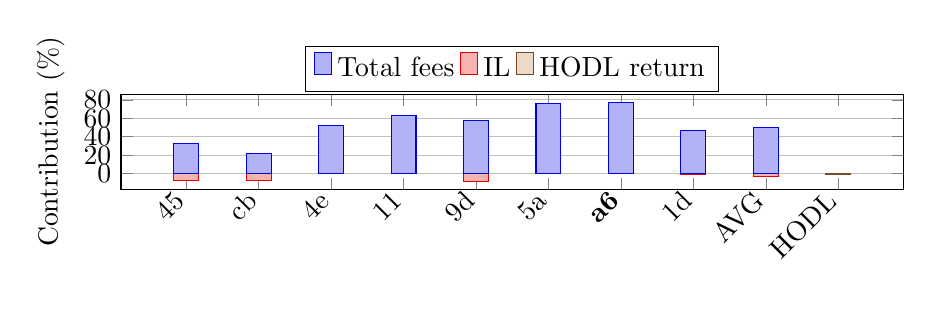
\begin{tikzpicture}
\begin{axis}[
    ybar stacked,
    width=0.95\linewidth,
    height=0.23\textwidth,
    bar width=9pt,
    ylabel={Contribution (\%)},
    symbolic x coords={45,cb,4e,11,9d,5a,a6,1d,AVG,HODL},
    xtick=data,
    xticklabels={45,cb,4e,11,9d,5a,\textbf{a6},1d,AVG,HODL},
    xticklabel style={rotate=45,anchor=east},
    ymajorgrids=true,
    legend style={at={(0.5,1.02)},anchor=south,legend columns=3},
]
\addplot coordinates {
  (45,32.53) (cb,21.93) (4e,52.60) (11,62.77) (9d,57.41) (5a,76.27) (a6,77.39) (1d,46.42)
  (AVG,49.99) (HODL,0.00)
};
\addlegendentry{Total fees}

\addplot coordinates {
  (45,-7.40) (cb,-7.36) (4e,-0.04) (11,-0.05) (9d,-8.44) (5a,-0.09) (a6,-0.01) (1d,-1.02)
  (AVG,-3.48) (HODL,0.00)
};
\addlegendentry{IL}

\addplot coordinates {
  (45,0.00) (cb,0.00) (4e,0.00) (11,0.00) (9d,0.00) (5a,0.00) (a6,0.00) (1d,0.00)
  (AVG,0.00) (HODL,-1.00)
};
\addlegendentry{HODL return}
\end{axis}
\end{tikzpicture}
\caption{Pool fees versus IL over 3.5 years (May~2022--Dec~2025).}
\label{fig:post_contrib}
\end{figure}

Taken together, \noindent\textit{Tables~\ref{tab:first_year_net90} to \ref{tab:case_bear_bull} and Fig.~\ref{fig:post_contrib} show that the proposed metrics support a practical decision workflow, rather than serving only as descriptive statistics}. 
Using only the first year for calibration, the rules identified a pool that delivered consistently positive \emph{excess} gains across opposite ETH/USD regimes and over a multi-year out-of-sample horizon. 
These results were further explained by decomposing excess gains into fee income and IL. 
Superior outcomes arose when strong fee velocity was paired with controlled divergence risk. 
By contrast, high-fee pools could still underperform when structural divergence dominated, as seen in stablecoin-anchored pairs during the drawdown window. 
Finally, we note that as both fee conditions and correlation regimes evolve over time, the workflow should be applied periodically (e.g., monthly or quarterly) using recent data.



\section{Conclusion}
\label{sec:conclusion}
In this paper, we study IL in Uniswap v3 to provide LPs with a practical, data-driven way to quantify IL risk and compare pools beyond simple fee-tier heuristics. 
Using multi-year pool data, we show that net outcomes are driven by the interaction of fee generation and divergence risk, motivating simple selection rules based on distributional IL summaries, tail bounds, and predictability diagnostics. 
Future work will extend the analysis to a broader pool universe across additional DeFi platforms and develop an adaptive fee policy that adjusts fees using rolling correlation and realized net performance to better match time-varying IL risk.

\section*{Acknowledgments}
\noindent\textbf{AI content disclosure.} The paper used OpenAI, Gemini, and Grammarly for language editing (grammar, clarity, and \LaTeX{}/formatting suggestions). The authors are responsible for the technical content and for verifying the final manuscript.


\bibliographystyle{IEEEtran}
\bibliography{references}

\end{document}